\documentclass[11pt]{lecturenotes}

%\let\theenumiorg\theenumi
%
%\newcommand{\code}[1]{\texttt{#1}}
\topsep 0pt
\itemsep 0pt

\usepackage{enumitem}
\usepackage{tikz}
\usetikzlibrary{arrows.meta}

\newcommand{\objExplainPrinciples}{\item explain the principles of survey design including question design, sampling, statistical inference, and sources of error}
\newcommand{\objDevelopQuestions}{\item explain the principles of survey design including question design, sampling, statistical inference, and sources of error}
\newcommand{\objAdvocate}{\item advocate for inclusion of measures on surveys using a scientific justification}
\newcommand{\objDataManagement}{\item conduct basic data management tasks and descriptive analysis in \textsf{R}}


\title{Semester Review}
\author{Michael Bader}
\week{14}
\lesson{1}
\coursenumber{SOCY 625}
\coursetitle{Practicum in Sociological Research}


\begin{document}
\maketitle

\begin{objectives}{
\item Define and explain inference, error (including validity, reliability, and bias), and variance
\item Identify sources of measurement error in survey design
\item Identify sources of representational errors in survey design
\item Explain the value of survey research for answering sociological questions
}{
\objExplainPrinciples
}
\end{objectives}

\section[15]{Questions about Memo}
Let's go back to the image that we have been using over and over again: 

\section{Review}
\subsection[20]{Major Concepts}
Review major concepts (have students try to define each term in succession with think-pair-share): 

\begin{itemize}
\item Inference
\item Error
	\begin{itemize}
	\item Validity
	\item Reliability
	\item Bias
	\end{itemize}
\item Variance
\end{itemize}

We can break down our understanding of these concepts into two types of inference as we have discussed throughout the class: \emph{measurement} and \emph{representation}. Let's start with measurement.

\begin{center}
\includegraphics{../../Week2-InferenceAndError/images/GrovesCh2Fig2.pdf}
\end{center}



\subsection[40]{Measurement}
Recall that in the figure, we go from the most ``pure'' representation of what we want to capture to the least pure. At each stage (each arrow), error creeps into the process. 

Let's start with the \emph{construct}. What is the construct?

\concept{construct}{elements of information sought by the researcher (Groves, et al., 41)}

How does the construct relate to theory? 

\concept{measurement}{how we ask our questions to measure our construct of interest}

What \emph{inferential errors} can creep into the measurement of our construct? In other words, what can reduce the \textbf{validity} of the measurement?

\concept{response}{how a respondent understands, interprets, and responds to our measurement (questions)}

\begin{center}
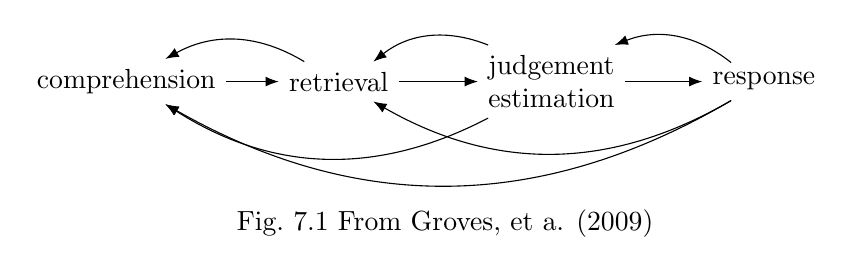
\begin{tikzpicture}[scale=.9]
\usetikzlibrary{arrows.meta}

\node [align=center, thick] (comp)  at (0,0) {comprehension};
\node [align=center, thick] (retr) at (3,0) {retrieval};
\node [align=center, thick] (judg) at (6,0) {judgement\\estimation};
\node [align=center, thick] (resp) at (9,0) {response};

\path [-Latex] (comp) edge (retr) (retr) edge (judg) (judg) edge (resp);
\draw [-Latex] (resp) to [bend right] (judg);
\draw [-Latex] (judg) to [bend right] (retr);
\draw [-Latex] (retr) to [bend right] (comp);
\draw [-Latex] (resp) to [bend left] (retr);
\draw [-Latex] (judg) to [bend left] (comp);
\draw [-Latex] (resp) to [bend left] (comp);

\node [align=center] at (4.5,-2) {Fig.\ 7.1 From Groves, et a. (2009)};

\end{tikzpicture}
\end{center}

\concept{edited response}{the response ultimately used in our analysis}

For example, the race and ethnicity questions that you recoded in R. 

Any questions? 


\subsection[40]{Representation}
The other side of the figure represents how we infer to populations based on sometimes very small samples from that population. Again, we go from the most ``pure'' concept, the target population, to the least pure as error gets introduced at each step of the process. 

\concept{target population}{group of elements (people) that we want to represent with our survey}

\concept{sampling frame}{the enumerated list of elements in the target population from which we will draw our sample}

How does error get introduced going from the target population to the sampling frame? 

What are the types of errors should cause us concern?

\concept{sample}{a subset of elements drawn from the sampling frame; in survey research, that should be based on a \emph{probabilistic sample}}

Good survey samples give (in theory): 

\begin{itemize}
\item All elements in the target population a non-zero probability of inclusion into the sample
\item All elements in the sampling frame have a known probability of inclusion into the sample
\item The elements of the sample are \emph{unbiased} with respect to the target population
\end{itemize}

\concept{sampling variation}{the amount of variation around a population value due to random chances of drawing different samples from a population}

Known values of sampling variation can only be calculated if the survey can be drawn using probabilistic samples.

Sampling variation (sampling error) will be \textbf{lower}:
\begin{enumerate}
\item with larger samples (though nonlinear)
\item with less variation in the measure
\end{enumerate} 

Samples of size: 
\begin{description}
\item[1] will have sampling variance equal to the variance of the measure
\item[N] will have no sampling variance equal to 0 
\end{description}

\begin{center}
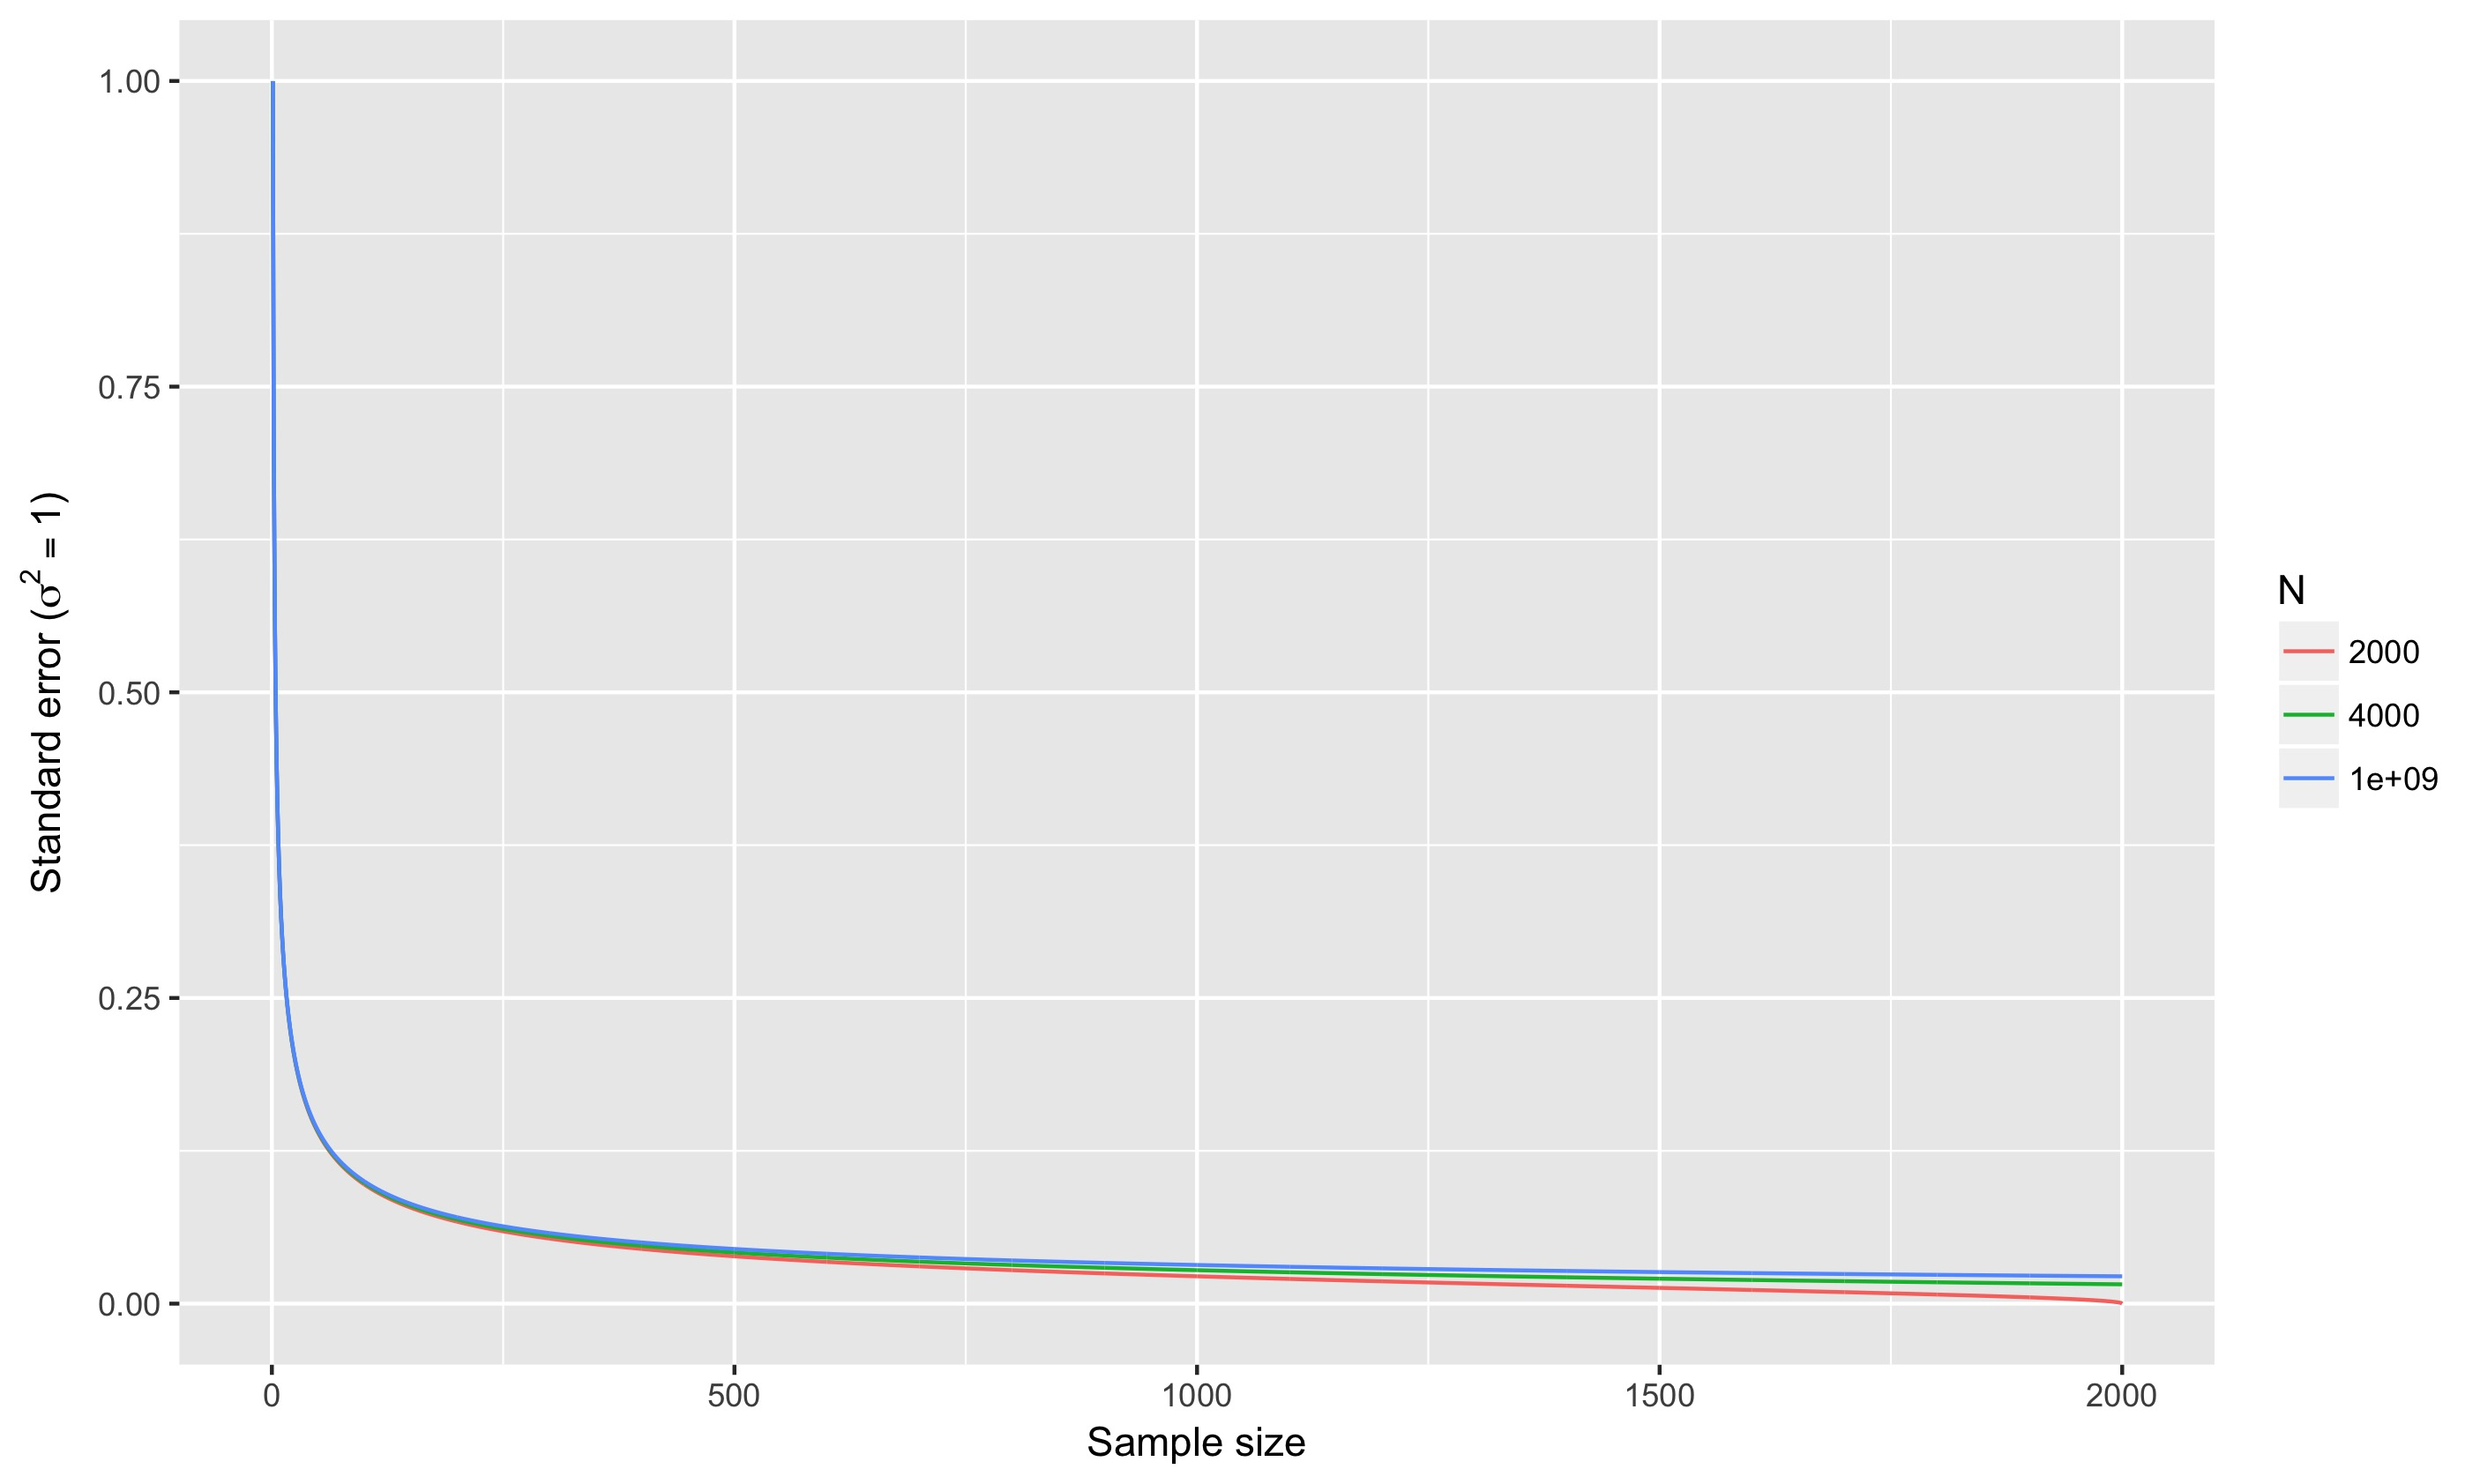
\includegraphics[width=4in]{../images/sampleSizePlot.jpeg}
\end{center}

\concept{respondents}{people who actually answer questions on our instrument}

\begin{itemize}
\item Unit non-response
\item Item non-response
\end{itemize}

\concept{survey weights}{assign values equal to the inverse of the probability that a particular unit responded to the survey given known quantities in the target population}

Important for design of samples to balance cost savings with representational inference. 

\begin{description}
\item[Clustered sample] Sample primary sampling units (PSUs) and then sample elements within those PSUs (tends to increase design effect)
\item[Stratified sample] Sample from different strata of the population to ensure representation (tends to decrease sampling variance)
\end{description}

\section[10]{Wrapping Up \& Moving Forward}
Surveys, when done right, offer a democratic form of data. That might sound highfalutin, but on questions of major concern, we offer everyone the chance to be heard when we use survey methods. Only through these methods can we infer information about the population at large. 

That doesn't mean it should be the only method that we use. We cannot get detailed information from any individual respondent. If we are not careful to involve communities, we can risk asking questions that do not help those outside of the academy. In an ideal world, we would use the accumulation of research from different methods to improve our knowledge of the world. 

I hope that when you read stories in the news or in academic journals, you get a sense of what goes into a quality survey. If you can't find information about how the journalist or researcher addressed measurement and representational inference, then you should be skeptical of the findings. 

At the same time, you have likely gained an appreciation for the skill and effort it takes to field a quality survey. After all, the survey statistic at the bottom of the flow chart represents something as simple as a sample mean. Think about all of the work that went into creating that one simple measure.

As we move forward, you should keep in mind all that you have learned in this class. Our models will become more complicated than a simple sample mean, but the principles that you learned about survey research will all be relevant to you future research. 

\end{document}
